\chapter{Transformation des données}
Toujours en partant de la preuve de concept réalisée par Florence Clavaud, la transformation automatique des données se fait en utilisant un unique programme écrit dans le langage XSLT 2.0.\footnote{Lien vers \href{https://www.w3.org/TR/xslt20/}{la spécification W3C.}} Le choix de ce langage tient au format de sortie choisi qui est RDF/XML. XSLT est une technologie extrêmement performante quand il s'agit de transformer du XML ou du texte en XML.
\section{Transformation à partir des tableaux Excel}
\subsection{Logique de transformation}
Pourquoi partir des données des fichiers Excel, et ne pas utiliser le logiciel RiC-O Converter sur les données en EAD ? En effet l'inventaire virtuel encodé en EAD contient déjà les données saisies dans les fichiers Excel de dépouillements. Tout d'abord, utiliser le logiciel RiC-O Converter aurait été complexe puisqu'il ne connaît pas l'extension de RiC-O que nous avons produite, il aurait donc fallu que nous nous l'approprions et l'adaptions à nos besoins. Et pourquoi ne pas partir du fichier EAD et faire notre script qui utilisera l'ontologie ORESM ? En fait, il s'avérait nettement préférable de partir de la source Excel : le fichier EAD résultait déjà d'une transformation simplifiant de beaucoup la structure initiale des données. Finalement il était plus naturel et plus rapide de partir de la base déjà fournie par la preuve de concept proposée par Florence Clavaud. 
\par
Pour gagner du temps nous avons utilisé le logiciel Oxygen\footnote{C'est à partir de la version 23 qu'Oxygen propose cette fonctionnalité directement incluse, pour des versions plus anciennes il faudra installer un add-on.} qui permet de transformer un fichier Excel en format XML. On se retrouve avec un fichier ayant un élément racine qui contient pour chaque ligne du tableau original un élément XML \textbf{<document>}. Dans chacun des éléments \textbf{<document>}, on trouve pour chaque colonne du tableau Excel, un élément du même nom qui contient la valeur de la cellule correspondante dans le tableau.
\begin{figure}[!h]
    \centering
    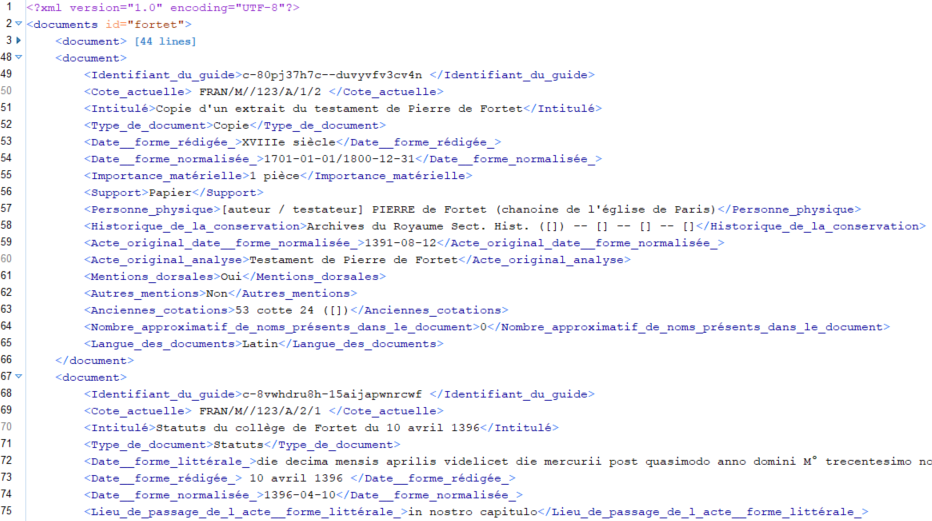
\includegraphics[width=1\linewidth]{images/tableau-fortet-xml.png}
    \caption{Premières lignes du fichier XML issu du tableau de dépouillement du collège de Fortet.}
    \label{fig:xml-fortet}
\end{figure}

\subsection{Organisation à la sortie du script}
Tout l'objectif du script est d'extraire de ces fichiers tabulaires la description des entités qui s'y trouvent mentionnées et qui sont dignes d'intérêt pour le projet, et les relations qui lient les entités entre elles pour former un graphe orienté. On change complètement la manière d'organiser les données. Selon l'approche déjà suivie par Florence Clavaud pour sa preuve de concept, le script traite en premier lieu les entités de contexte et seulement à la fin du processus, les documents. La relation entre ces entités de contexte et le document décrit est exprimée au moment où les entités de contexte sont traitées. Pour bien différencier les types d'entités chacun bénéficie de son propre fichier de sortie. Il en résulte :
\begin{itemize}
    \item Un fichier pour les personnes physiques (3478 entités rico:Person créées).
    \item Un fichier pour les personnes morales (102 entités rico:CorporateBody).
    \item Un fichier pour les lieux (314 entités rico:Place).
    \item Un pour les cotes anciennes et un pour les cotes actuelles (2745 rico:Identifier).
    \item Un fichier pour les types d'activité, de titre, ou de fonction (929 rico:OccupationType).
    \item Un fichier pour les dates (1715 entités date).
    \item Un fichier unique pour les statuts et types de documents (120 entités rico:Type).
\end{itemize}
\par
L'URI de chaque entité créée par le projet ORESM commence par une chaîne de caractères invariante déclarée dans les fichiers XML/RDF de sortie, \og  http://data.oresm.fr\fg. Dans le cas des entités ci-dessus l'URI est suivi par la classe puis le nom de l'entité. Donc  l'URI du lieu Paris est \og http://data.oresm.fr/place/Paris\fg. 
\par
Pour l'entité représentant le document d'archives le fichier de sortie est individualisé. Pour nous retrouver dans la masse de ces fichiers (1445 fichiers, un fichier par document dépouillé) il a fallu trouver un moyen pour les différencier. Nous avons décidé de créer une clé d'identification à partir du numéro d'ordre de la ligne décrivant le document dans le tableau, et du nom du fichier d'origine. Ainsi le document  qui est décrit à la ligne 145 du fichier relatif au collège de Fortet est décrit en RDF dans le fichier de sortie \og document-fortet-145\fg . C'est un très bon moyen court et efficace pour se retrouver en utilisant autre chose que la cote ou l'analyse. C'est d'ailleurs sur cette même logique que sont construits les URI des documents. Toujours en reprenant l'exemple précédent, l'URI des deux entités RiC-O représentant le document décrit à la ligne 145 est recordResource/or-fortet-145 et instantiation/or-fortet-145 (le radical or signifie ORESM). Ce système d'identification permet de cibler un document très précisément, et de le retrouver très rapidement, notamment dans le script, lorsqu'on exprime la relation entre l'entité de contexte et le document, il suffit simplement d'identifier la ligne.


\section{Commentaires}
\subsection{Réussites}
En premier lieu il est important de souligner la réussite de cette étape. Le script XSLT remplit parfaitement son mandat. En suivant le tableau de mapping, chaque cellule d'origine des tableaux est transformée en RDF suivant l'ontologie RiC-O/ORESM. Le script produit les fichiers de sortie en moins de 10 secondes. C'est la une force de XSLT, la vitesse d'exécution. La plus grosse difficulté a été de gérer les actes et leurs originaux, notamment pour éviter les doublons, quand deux actes sont la copie d'un même original. En quelques mots, quand un acte est issu d'un original également décrit via une ligne d'un fichier Excel, on peut regrouper les données décrivant cet unique original et ne créer au final qu'une seule description de cet original, en utilisant les champs concernant sa cote. Quand l'original n'est pas dans les actes dépouillés alors il est créé une entité RecordResource représentant l'acte original mais sans entité Instantiation associée. C'est ce que nous avons appelé un acte \og virtuel\fg. 
\par
Mais il est possible que plusieurs actes soient tirés d'un même original, pas encore dépouillé, voire même perdu. Pour éviter les doublons d'actes virtuels, il a été décidé de comparer les données \textbf{Acte\_original\_analyse} et \textbf{Acte\_original\_date}. Si l'archiviste a relevé la même date et la même analyse pour la pièce originale de deux (ou plus) documents lors du dépouillement, alors on considère qu'ils sont issus de la même pièce. Pour illustrer cette situation prenons les pièces ayant pour cote, l'une \textbf{FRAN/M//74/9} et l'autre \textbf{FRAN/M//74/10}. Pour ces deux pièces l'archiviste a relevé que l'original était daté de \textit{1263-05-04} et a rédigé une analyse identique \footnote{\textit{Privilège donné aux pauvres maîtres de Sorbonne par le pape Urbain le 4 des nones de mai l’an II de son pontificat de construire une chapelle et d’y célébrer les offices.}}. Dans un tel cas, le script ne crée qu'un unique acte virtuel. Cette logique permet de de faire émerger des clusters de relations. Pour donner une idée, dans nos données, un acte virtuel a pu être lié à neuf actes dépouillés. Il a aussi été décider d'effectuer la normalisation\footnote{Au format ISO 8601 : yyyy-mm-dd} des formes rédigées des dates quand celles-ci répondent à un certain schéma, identifié à l'aide d'expressions régulières\footnote{Les expressions régulières sont des motifs de recherche qui permettent de décrire des modèles de chaînes de caractères. Voir la page wikipédia dédiée \href{https://fr.wikipedia.org/wiki/Expression\_r\%C3\%A9guli\%C3\%A8re}{https://fr.wikipedia.org/wiki/Expression\_régulière}.}. Le script ne réalise donc pas uniquement une transformation mais effectue un traitement et une interprétation des données quand il est intéressant de le faire.

\subsection{Limites}
Évidemment on ne peut pas tout faire dans un unique script. Certains traitements qui auraient pu être envisagés ont été laissés de côté. 

\subsubsection{Pas de réconciliation précise des entités nommées}
Concernant les entités nommées, la seule réconciliation opérée consiste à regrouper les entités sur la base d'une égalité parfaite des valeurs qui les concernent. Les entités de type personne (appartenant à la classe Person de RiC-O) sont regroupées sur leurs noms mais aussi leurs occupations. Ainsi un \og Germain Gouffe \fg identifié dans un acte comme "écolier de l'université de Paris" et \og Germain Gouffe\fg, identifié dans un autre comme "\textbf{pauvre} écolier de l'université de Paris" ne seront pas considérés comme la même personne. La complexité des conditions mises en place pour s'assurer qu'une personne identifiée dans un document est bien la même que dans un autre nous a motivé à reporter ce traitement. En limitant au maximum les regroupements nous avons voulu empêcher les erreurs qui pourraient pénaliser un futur traitement. Mais il ne faut pas imaginer qu'il n'y en a aucune. Il ne faudra pas l'oublier lorsque viendra le temps de s'attaquer au traitement de la masse de noms extraits des dépouillements. Nous pourrons envisager d'utiliser des outils plus adaptés à l'alignement de données comme Dataiku\footnote{\href{https://www.dataiku.com/}{https://www.dataiku.com/}} ou Open Refine\footnote{\href{https://openrefine.org/}{https://openrefine.org/}}.
\par
Il semble tout de même important de signaler, notamment en ce qui concerne certains lieux, que les données ne se prêtent absolument pas à un regroupement. Certains noms de lieux relevés dans les actes n'ont été consignés que sous leur forme littérale et n'ont pas été normalisés avec un nom bien identifiable et des éléments de localisation. Par conséquent, certains des noms ne sont absolument pas exploitables. Particulièrement pour les formes littérales qui expriment un lieu relatif (\textit{in nostro capitulo\footnote{\textit{dans notre chapitre}}}, \textit{audict colleige}), ce regroupement, qui s'effectue quand même, ne fait pas de sens pour ces valeurs. Il y aura un travail a effectuer pour corriger les données en amont de la transformation.
\subsubsection{Des limites aperçu dans la méthodologie}
Une seule colonne des tableaux de dépouillements n'a pas pu être traitée dans son intégralité, c'est le champ \textbf{Remarques}. Nécessairement un champ aussi libre, dans la nature de son contenu, ne pouvait qu'entraîner des problèmes dans un modèle entité relation. Les remarques de l'archiviste ne concernent pas uniquement la pièce dépouillée mais parfois concernent la cote, les personnes, la date, le lieu etc. Impossible pour le script d'identifier à quelle entité se rapporte la remarque, d'autant plus que la structure des valeurs de cette colonne n'est pas totalement régulière en fonction du contenu. Un tableau a été construit pour imaginer une typologie des remarques par rapport à l'entité RiC-O à laquelle elles se rapportent. Nul doute qu'il faudra revoir la manière dont la méthodologie prévoit la saisie de ces remarques pour permettre au script de les exploiter. 